\documentclass[12pt, letterpaper]{article}
\usepackage{polski}
\usepackage[utf8]{inputenc}
\usepackage{array}
\usepackage[top=2cm]{geometry}
\usepackage{fancyhdr}
\usepackage{graphicx}
\usepackage{longtable}
\renewcommand{\arraystretch}{1.2} %table height x1.5

\title{
    \textbf{PROJEKT \\ [.3cm] % .3cm of space below
    \large System wspomagający wzmacnanie odporności psychicznej} \\ [.4cm]
    \date{}
    \author{}
}

\begin{document}

    \setlength{\headheight}{15pt}
    \pagestyle{fancy}
    \fancyhead{} % clear all header fields
    \fancyhead[R]{\textbf{GoodMentality}}
    \fancyhead[C]{\date{\today}}
    \fancyhead[L]{SCRUM: Backlog produktu}
    \fancyfoot{} % clear all footer fields
    \fancyfoot[R]{\thepage}
    \fancyfoot[L]{DP-05042023-2}

    \begin{titlepage}
        \maketitle
        \thispagestyle{empty} % excludes page number from the first page
        \begin{center}
            \begin{tabular}{  m{0.8\textwidth}  } 
                \hline 
                \Large Tytuł: SCRUM - Backlog produktu \\ %title
                \hline
            \end{tabular}

            \vspace{1.5cm}

            \fbox{
                \parbox{\textwidth}{
                    Streszczenie: Celem zadania jest opisanie produktu wytwarzanego w 
                    ramach projektu. Produkt przybliżany jest poprzez biznesowy scenariusz 
                    jego użycia (ang. business scenario), z którego następnie wywodzone 
                    są cechy produktu (funkcjonalne i pozafunkcjonalne) dokumentowane 
                    w backlogu produktu (ang. product backlog, PB) z priorytetami.  %streszczenie here
                    }
                }

            \vspace{1.5cm}

            \begin{tabular}{ | m{0.25\textwidth} | m{0.73\textwidth}|  } 
                \hline
                Wersja: & 1.0 \\ %Version before '\\'
                \hline
                Data wydania: & \date{\today} \\ %Date before '\\'
                \hline
                Redaktor: & Szymon Hejmanowski \\ %Author before '\\'
                \hline
                Współautorzy: & Patryk Gołembiewski \\ %Coauthors before '\\'
                \hline
                Etap: & 2 \\ %Stage before '\\'
                \hline
                Nazwa pliku: & DP-05042023-2 \\ %File name before '\\'
                \hline
                Liczba stron: & \\ %Page number before '\\'
                \hline
                \end{tabular}
        \end{center}    
    \end{titlepage}

    \tableofcontents

    \pagebreak

    \section{O projekcie i produkcie}
    Produktem naszego zespołu ma być aplikacja GoodMentality zapewniająca wsparcie 
    w budowie odporności psychicznej. Osobami korzystającymi z systemu będą
    osoby zainteresowane tematem poprawy swojego życia poprzez zadbanie o sfere
    mentalną. Produkt ma składać się z poszczególnie wyselekcjonowanych funkcjonalności
    z których każda oddziałowywuje na pewny obszar zawarty w modelu 4C.


    \section{Persony użytkowników}
    W celu stworzenia persony użytkownika posłużyliśmy się metodą \textbf{mapy empatii}. Zakłada
    ona opisanie osoby poprzez odpowiedzi na szereg pytań dotyczących jego zachowania, 
    odczuć oraz emocji. \\

    \begin{figure}[h]
        \centering
        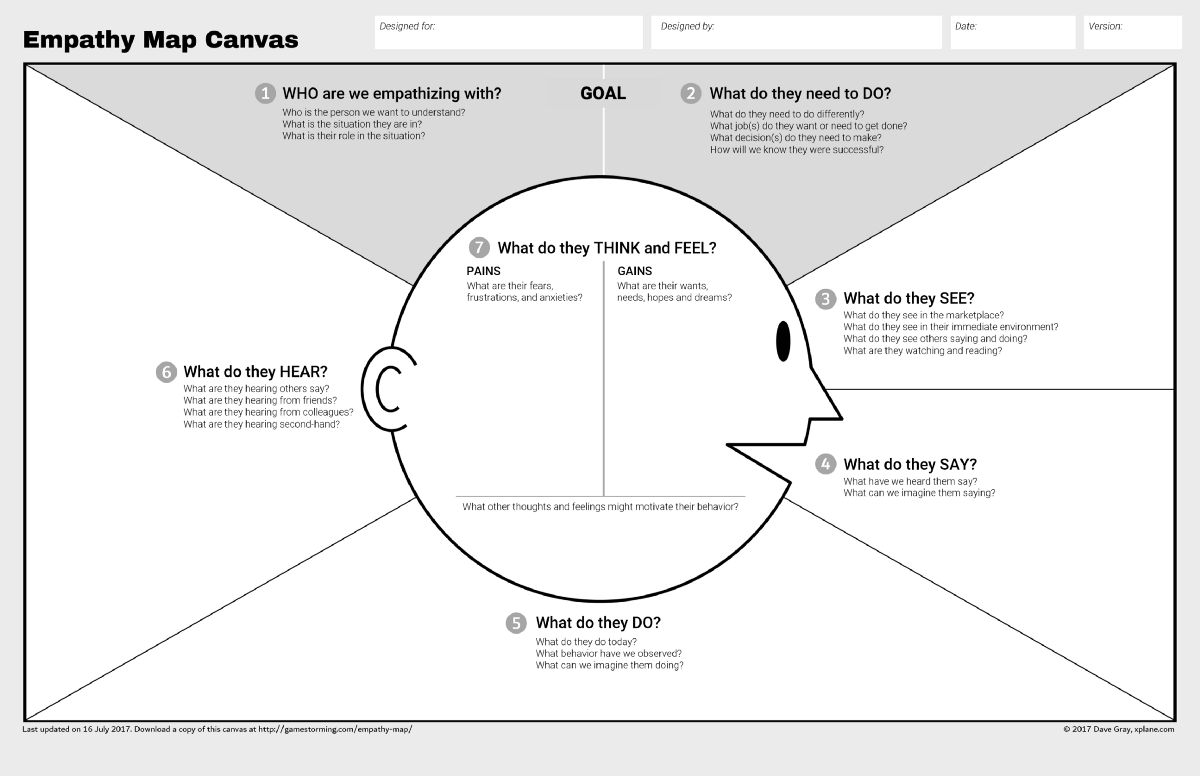
\includegraphics[width=\textwidth]{empathymap.png}
        \caption{Przykładowa mapa empatii.}
    \end{figure}

    \pagebreak

    \subsubsection*{Who are we empathizing with?}
    Osoba, która chce poprawić swoją odporność psychiczną. Osoba taka mierzy się na co 
    dzień z wieloma wyzwaniami i problemami chce być w stanie zwalczać je z większą 
    łatwością oraz mieć większy komfort psychiczny.

    \subsubsection*{What do they need to do?}
    Zapoznać się z aplikacją. Nauczyć się jej obsługi. Uzupełnić cele długoterminowe.
    Codziennie zaglądać do aplikacji, aby uzupełnić dziennik oraz wyznaczyć cele na kolejny dzień. 

    \subsubsection*{What do they see?}
    Na co dzień widzi świat pełen trudności i problemów. Niezliczoną ilość przytłaczających 
    wyzwań. W Internecie widzi innych, którzy cieszą się życiem i wydają się nie posiadać 
    żadnej troski. Widzi ciągłe zmiany do których nie jest w stanie przywyknąć oraz ludzi, 
    z których każdy wydaje się obcy.

    \subsubsection*{What do they say?}
    Mówi, że nie jest w stanie sobie poradzić z codziennością. Narzeka na nieustające trudności. 
    Mówi, że nie czuje kontroli nad własnym życiem.

    \subsubsection*{What do they do?}
    Stoi w miejscu, pragnąc zmiany. Nie jest w stanie jednak niczego wskórać. Codziennie 
    obiecuje sobie, że zrealizuje postawione cele, jednak jest to tylko złudne poczucie. 
    Każdego dnia idzie spać o innej porze, przez co nie jest w stanie się wyspać. 
    Nie pielęgnuje relacji z bliskimi. Jest reaktywna, zarówno w życiu zawodowym 
    jak i osobistym. Nie pomaga innym.

    \subsubsection*{What do they hear?}
    Od innych słyszy, że musi wziąć się w garść i zrobić coś ze swoim życiem. 
    Docierają do niej stale słowa krytyki od innych. Koledzy namawiają ją na 
    wyjścia jednak ona nie ma siły ani ochoty wychodzić z domu.  

    \subsubsection*{What do they think and feel?}

    \begin{center}
        \begin{tabular}{ | m{0.5\textwidth} | m{0.5\textwidth} | }
            \hline
            Pains & Gains \\ 
            \hline
            Ma lęk przed tym, że nie będzie w stanie zrealizować 
            wszystkich zadań oraz, że nie radzi sobie z codziennymi 
            problemami. Jest sfrustrowana swoją postawą i ciągłym 
            brakiem poprawy. Boi się, że przez swoje zaniedbywanie 
            kontaktów oraz złe nastawienie odwrócą się od niej znajomi. 
            Obawia się o swoje zdrowie fizyczne z powodu zaniedbywania 
            sfery somatycznej egzystencji. & 
            Ma nadzieję, że walka z codziennymi trudnościami będzie dla 
            niej łatwiejsza. Chciałaby z uśmiechem stawiać czoła 
            kolejnemu dniu. Zależy jej również na poprawie relacji 
            z ludźmi. Liczy, że jej zdrowie fizyczne również się 
            poprawi. Chciałaby mieć pełną kontrolę nad swoim życiem 
            oraz większą pewność siebie. Obecnie czuje złość, że nie
            jest w stanie realizować swoich postanowień.
            \\
            \hline  
        \end{tabular}
    \end{center}
    

    \section{Scenariusz użycia produktu}
    Scenariusze użycia zostały stworzone zgodnie z schematem \textbf{AS IS - TO BE}. Każda
    z funkcjonalności produktu uzyskała osobny scenariusz.

    \begin{center}
        \begin{longtable}{ | m{0.5\textwidth} | m{0.5\textwidth} | }
            \hline
            AS IS & TO BE \\ 
            \hline
            Osoba szybko zniechęca się do wykonywanych zadań, ponieważ nie czuje
            namacalnego progresu. Przez to, że myśli jedynie o tym co ma jeszcze
            do wykonania (a nie odnotowuje ile już zrobiła)  ma ciągłe wrażenie
            braku postępu, co ją wysoce demotywuje. Brak kontroli oraz
            zaangażowania. & MOsoba szybko zniechęca się do wykonywanych zadań,
            ponieważ nie czuje namacalnego progresu. Przez to, że myśli jedynie
            o tym co ma jeszcze do wykonania (a nie odnotowuje ile już zrobiła)
            ma ciągłe wrażenie braku postępu, co ją wysoce demotywuje. Brak
            kontroli oraz zaangażowania. \\
            \hline
            Osoba nie ma jasno wyznaczonych i skonkretyzowanych celów do jakich
            dąży. Chce schudnąć jednak nigdzie nie odnotowała ile i w jakim
            czasie. Przez to, że cel jest bardzo ogólny i bez wyznaczonego
            terminu, jest on tak naprawdę jedynie marzeniem. Osobie tej, wydaje
            się, że od czasu do czasu zje mniej lub pójdzie pobiegać, więc dąży
            do realizacji celu, jednak nie zdaje sobie sprawy, że wykonywana
            praca jest wyraźnie zbyt mała aby odnieść rezultat. Tkwi w
            przekonaniu, że dąży do celu, jednak w rzeczywistości jedynie stoi w
            miejscu. Taki status quo w dziedzinie jej celów obniża jej pewność
            siebie, ma wrażenie, że jest gorsza od innych bo też pracuje, jednak
            bez rezultatu. Dodatkowo traci poczucie kontroli, ma wrażenie, że
            nie ma wpływu na to co się dzieje w jej życiu. Nie jest w stanie
            realnie się zaangażować. Również taki stan negatywnie wpływa na
            obszar wyzwań z modelu 4C – nigdy nie ponosi jednoznacznej porażki
            (ponieważ jej cel nie ma terminu ani konkretnych założeń), z której
            mogłaby wyciągnąć lekcje, a jednocześnie nigdy nie osiąga celu.  &
            Osoba dodaje nowy cel w aplikacji zgodnie z formularzem. Podaje tam
            obiektywne i mierzalne wartości, które chce osiągnąć (konkretna
            waga, ilość pieniędzy jakie chce zarobić, ilość materiału do
            nauczenia) oraz termin realizacji tych zadań. W obszarze celu może
            również ustawić tak zwane milestones, czyli cele pośrednie, które są
            kluczowe do osiągnięcia ostatecznego celu. Widok bliższego celu
            pośredniego na horyzoncie daje jej dużą motywacje na początku i
            podtrzymuje ją w momentach zwątpienia. Osoba ta ma realne cele i w
            pełni świadomie dąży do nich każdego dnia. Osoba widząc postęp w
            kolejnych celach zyskuje poczucie kontroli nad sobą oraz własnym
            życiem. Pozwala jej się to również zaangażować i trwać w swoich
            postanowieniach. Jeśli któregoś z celów nie wypełni, zdaje sobie
            sprawę ze swojej porażki co pozwala jej wyciągnąć lekcje, wpływa to
            dobrze na obszar Wyzwania. Większa kontrola oraz widoczny rozwój
            zwiększa jej pewność siebie i przekłada się pozytywnie na inne
            obszary. \\
            \hline  
            Osoba ma skłonności do pesymizmu, lubi się zamartwiać i znajdować we
            wszystkim jedynie negatywy. Jest to dla niej demotywujące i zabija w
            niej chęć rozwoju. Osoba twierdzi, że rozwój i tak nic nie zmieni i
            że w ogóle jest bezsensu. & Aplikacja zapewnia osobie codzienne
            cytaty motywujące oraz inspirujące myśli tych, którzy wiele
            osiągnęli. O ile nie wpływa to z dnia na dzień na osobę, to jednak w
            dłuższym okresie czasu pozwala jej unikać pułapki ciągłego pesymizmu
            i odżywia jej mózg pozytywnymi myślami. \\
            \hline
            Osoba przez lata złych nawyków kształtowanych przez system szkolny
            oraz własne zaniedbania ma duże problemy ze snem. Nie zdaje sobie
            sprawy z tego, na jak wiele obszarów zdrowia oraz pracy mózgu on
            wpływa. Zaniedbuje sen sypiając w różnych godzinach oraz często
            niewystarczająco długo. Ma problemy z przyswajaniem i
            zapamiętywaniem, również pamięć mięśniowa na tym traci, przez co np.
            nauka gry na fortepianie staje się dla niej dużo trudniejsza.
            Odczuwa również negatywne skutki słabej higieny snu poprzez częste
            przeziębienia. Nierzadko musi odpuszczać przez to treningi lub
            wyjścia ze znajomymi. Ma poczucie braku kontroli nad własnym
            zdrowiem. Dodatkowo trudności w przyswajaniu informacji oraz w nauce
            nowych czynności fizycznych zmniejszają jej pewność siebie. & Dzięki
            modułowi poprawy snu osoba może dowiedzieć się o tym jak ogromne
            skutki ma jego zaniedbywanie. Dzięki przejrzeniu panelu poświęconemu
            krótkim informacją z badań o negatywnych skutkach niepoprawnego snu
            znajduje potencjalne rozwiązanie swoich wielu problemów. Motywuje ją
            to do działania w tym obszarze życia. Ustala w aplikacji harmonogram
            snu, co skutkuje codziennymi przypomnieniami i/lub blokowaniem
            innych aplikacji w odpowiednich godzinach. Sprawdza również panel
            zapewniający krótkie porady o tym jak zadbać o dobrą jakość snu
            (zmniejszenie temperatury pokoju, przygotowanie do snu poprzez
            zmniejszenie tętna). Poprawa ilość oraz jakości snu wpływa
            pozytywnie na każdy aspekt życia osoby. Lepiej działający układ
            immunologiczny redukuje często liczbę przeziębień, dzięki czemu
            osoba nie musi opuszczać treningów i innych aktywności. Osoba
            przyswaja więcej materiału i pamięta go lepiej, co również redukuje
            czas jaki musi poświęcać na naukę. Dodatkowo nauka gry na
            fortepianie idzie nagle zauważalnie lepiej. Osoba zyskuje pewność
            siebie oraz poczucie kontroli nad własnym życiem i zdrowiem. \\
            \hline
            Osoba ma problemy ze skupieniem. W każdej wolnej chwili przegląda
            social  media lub ogląda seriale. Nie pozostawia jej to praktycznie
            żadnego czasu na uspokojenie myśli. Jedyny czas kiedy jest sama ze
            swoimi myślami to moment kiedy kładzie się spać. Nie pozwala jej to
            wyłączyć się i spokojnie zasnąć. Skupienie się przez dłuższy moment
            na pracy głębokiej lub na czynności nie dostarczającej do mózgu
            dużych ilości bodźców jest dla niej praktycznie nierealne. Przy
            nudnych aktywnościach odruchowo co chwilę sięga po telefon. Podczas
            czytania książki, osoba się irytuje, musi wielokrotnie czytać każde
            zdanie ponieważ co chwilę jej myśli pędzą w inną stronę. Ciągła
            praca mózgu na wysokich obrotach powoduje u osoby niepokój. Nie jest
            nawet do końca świadoma z czego on wynika, jednak wyraźnie go
            odczuwa z różną intensywnością na przestrzeni dnia. Osoba taka nie
            ma poczucia kontroli nawet nad własnymi myślami. Nie jest w stanie
            zaangażować się w pracę którą wykonuje. & Dzięki użytkowaniu
            aplikacji z wyszczególnieniem modułu medytacji / pracy nad oddechem,
            osoba zaznaje każdego dnia parunastu minut uspokojenia myśli. Jest w
            stanie codziennie pracować nad swoją uważnością. W jej głowię
            zaczynają pojawiać się nowe myśli. Po pewnym okresie codziennej
            medytacji niepokój osoby stopniowo zanika, jest ona w stanie o wiele
            łatwiej i lepiej skupić się na wykonywanych czynnościach. Często
            zdarza jej się wchodzić w tryb „flow”. Czynności której wcześniej
            wydawały się nudne (np. czytanie książki), teraz sprawiają jej
            przyjemność. Na co dzień nie ma wrażenie ciągłej gonitwy myśli, jest
            w stanie być bardziej obecna w danej chwili. Spokojny i uważny umysł
            pozytywnie przekłada się również na zasypianie. Przed snem osoba
            korzystając z aplikacji uspokaja myśli i kładzie się do snu w
            idealnym stanie. Osoba zyskuje dużo lepsze poczucie kontroli oraz
            jest w stanie angażować się w codzienne wyzywania. \\
            \hline
            Osoba przechodzi przez każdy kolejny dzień bez refleksji, nie zwraca
            uwagi na to jakie wydarzenia z dnia wpływają na jej samopoczucie.
            Często popełnia te same błędy ponieważ nie poświęca czasu na
            przemyślenie ich i znalezienie rozwiązania. Nie jest do końca
            świadoma swoich własnych emocji. Wraca w głowie do przeszłości
            jednak nie w celu jej analizy i wyciągnięcia wniosków, lecz w celu
            rozmyślań nad tym co by było gdyby postąpiła inaczej. Tworzy w ten
            sposób negatywne nastawienie do swojej własnej osoby jednocześnie
            nic nie zyskując. Traci pewność siebie. & Osoba z użyciem aplikacji
            poświęca codziennie chwilę by przeanalizować miniony dzień. Zapisuje
            problemy jakie wystąpiły danego dnia oraz znajduje ich rozwiązania /
            sposoby na uniknięcie w przyszłości. Jeśli dany problem pojawiał się
            kolejny raz, myśli nad tym dlaczego poprzednie rozwiązanie było
            nieskuteczne i jak je poprawić / zmienić. Ocenia również swoje
            samopoczucie na koniec dnia, dzięki czemu zyskuje świadomość co tak
            naprawdę wpływa na jej odczucia. Dzięki widocznej eliminacji błędów
            oraz świadomości emocji czuje, że zyskuje pewność siebie oraz
            kontrole. \\
            \hline
            Osoba każdego dnia budzi się bez konkretnych założeń co do tego co
            chciałaby zrobić. Ma w głowie zarys planów na dzień, jednak  są one
            nieskonkretyzowane. W dni w które ma wiele zadań nie czuje
            potrzebnej presji, przez co dzień nie jest optymalny i nie wyrabia
            się ze zrobieniem wszystkiego co powoduje stres i niezadowolenie. W
            dni, kiedy ma mało zadań i dużo czasu, zamiast skorzystać z
            możliwości i zaplanować ciekawą aktywność na ten dzień lub wykonać
            jakąś pracę na zapas, traci pół dnia na bezproduktywne czynności.
            Nie ma poczucia kontroli nad własnym dniem, nie jest w stanie
            optymalnie wykonywać swoich wyzwań oraz nie jest tak zaangażowana
            jakby mogła być. & Osoba codziennie wieczorem po wypełnieniu
            dziennika samopoczucia przechodzi do sekcji planowania następnego
            dnia. Na spokojnie zbiera wszystkie rzeczy, które powinna jutro
            zrobić i tworzy z nich listę. Nadaje im priorytety, szacunkowy czas
            wykonania oraz godziny. Widzi czy jest na niedoczasie i musi jutro
            wyjątkowo się wysilić czy może ma trochę wolnego czasu aby wyjść na
            kawę ze znajomymi. Następnego dnia od rana skoncentrowana jest na
            wypełnianiu zadań. Daje jej to duże poczucie satysfakcji co ułatwia
            przystępowanie do kolejnych zadań. Dzięki przydziałowi na każde
            zadanie swojego czasu jest w stanie skupić się na obecnie
            wykonywanej czynności. Dodatkowo świadomość na jakim etapie pracy
            jest w ciągu dnia redukuje w dużym stopniu jej stres i niepokój.
            Odhaczenie ostatniego zadania w trakcie danego dnia powoduje wyrzut
            dopaminy i zachęca do powtórzenia cyklu dnia kolejnego. \\
            \hline
        \end{longtable}
    \end{center}


    \section{Backlog produktu}
    Kolejność elementów Backlogu zgodna jest z ich priorytetami.
    \begin{figure}[h]
        \centering
        \includegraphics[width=\textwidth]{backlog.jpg}
        \caption{Backlog produktu wygenerowany za pomocą Jira.}
    \end{figure}

    \begin{figure}[h]
        \centering
        \includegraphics[width=\textwidth]{priority.jpg}
        \caption{Wyjaśnienie oznaczeń priorytetu.}
    \end{figure}


    \section{Definicja ukończenia}

    \begin{itemize}
        \item Wszystkie funkcjonalności z backlogu produktu zostały
        zaimplementowane i działają poprawnie. 

        \item Interfejs aplikacji jest intuicyjny i łatwy w obsłudze, zapewnia
        wygodny dostęp do wszystkich modułów i funkcjonalności. 

        \item Aplikacja jest dostępna w dwóch językach: polskim i angielskim. 

        \item Aplikacja spełnia wymagania prawa i polityki prywatności. 
        
        \item Aplikacja działa stabilnie i nie powoduje żadnych błędów lub
        awarii. 
        
        \item Aplikacja działa sprawnie i szybko, bez długiego czasu ładowania. 
        
        \item Aplikacja spełnia wszystkie wymagania użytkowników i zapewnia
        wysoką jakość usług. 
        
        \item Aplikacja jest zaprojektowana w taki sposób, aby zapewnić
        użytkownikowi kompleksowe wsparcie w wzmacnianiu odporności psychicznej. 
        
        \item Aplikacja jest zoptymalizowana pod kątem różnych rodzajów urządzeń
        mobilnych i działa poprawnie na różnych systemach operacyjnych. 
        
        \item Aplikacja jest w pełni przetestowana i spełnia standardy
        jakościowe. 
        
        \item Aplikacja jest zgodna z przepisami i standardami branżowymi. 
      \end{itemize}

    \pagebreak

    \section{Kryteria akceptacji}

    \begin{figure}[h]
        \centering
        \includegraphics{form.jpg}
        \caption{Kryteria akceptacji: formularz do wprowadzania nastroju.}
    \end{figure}

    \begin{figure}[h]
        \centering
        \includegraphics{hasla.jpg}
        \caption{Kryteria akceptacji: moduł haseł motywacyjnych.}
    \end{figure}

    \begin{figure}[h]
        \centering
        \includegraphics{notifications.jpg}
        \caption{Kryteria akceptacji: powiadomienia.}
    \end{figure}

    \begin{figure}[h]
        \centering
        \includegraphics{planer.jpg}
        \caption{Kryteria akceptacji: planer dnia.}
    \end{figure}

\end{document}